\documentclass{Phyport}

\usepackage{placeins}
\usepackage{hyperref}
\hypersetup{
    colorlinks=true,
}

\exname{光的偏振应用研究} %实验名称
\extable{8}
\instructor{姚星星} %指导教师
\class{github} %班级
\name{MJ} %姓名
\stuid{2025} %学号

\nyear{2025} %年
\nmonth{12} %月
\nday{1} %日
\nweekday{一} %星期几

\begin{document}
\setcounter{page}{0}
\makecover

\section{预习报告（10分）}
\subsection{实验综述（5分）}

光是一种电磁波和横波，能够朝着不同方向振荡的性质。当自然光入射到介质表面时，反射光就表现出一定的偏振性，
用菲涅耳公式描述，对于光矢量垂直于入射面的分量：
\begin{figure}[htbp!]
    \centering
    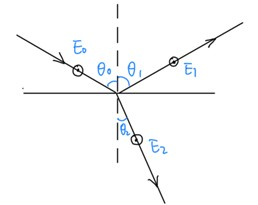
\includegraphics[width=0.2\textwidth]{demo1.jpg}
\end{figure}

\[
\frac{E_1}{E_0} = - \frac{\sin{(\theta_0 - \theta_2)}}{\sin{(\theta_0 + \theta_2)}}
\]

对于光矢量平行于入射面的分量：
\begin{figure}[htbp!]
    \centering
    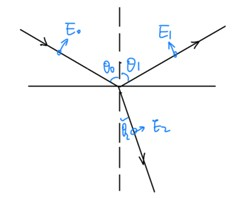
\includegraphics[width=0.2\textwidth]{demo2.jpg}
\end{figure}

\[
\frac{E_2}{E_0} = \frac{\tan{(\theta_0 - \theta_2)}}{\tan{(\theta_0 + \theta_2)}}
\]

当入射角达到布儒斯特角时，光矢量平行于入射面的分量接近零，反射光几乎完全呈线偏振，当介质的折射率为 $n$ 时，
其入射角满足：
\[
\tan{\theta_0} = n
\]

实验时通过观察反射光经偏振片后的光强变化并测量光的偏振程度的极大位置，就可以计算材料的折射率。

为了分析偏振态本身，还需要对偏振片的偏振化方向进行校准。实验中光以布儒斯特角 $\phi$ 入射黑色平板后成为线偏振光，
再经过偏振片时，透射光强随偏振片透光轴夹角变化，满足马吕斯定律：
\[
I = I_0 \cos^2{\phi}
\]

通过光电流信号大小寻找透射光强最小的位置，即可确定偏振片透光轴的方向。

在研究硅光电池特性时，可以通过旋转偏振片精确改变光照强度，从而测量硅光电池输出光电流随光强的变化规律，
发现基本满足线性关系。


\subsection{实验重点（3分）}

本实验的学习重点在于理解偏振光的产生、特点和应用以及菲涅尔公式的描述，掌握利用布儒斯特角测量材料折射率和马吕斯定律确定偏振片透光轴方向的方法，
以及了解硅光电池的光电流与光强的特性。

\subsection{实验难点（2分）}

本实验的实现难点主要在于黑色平板的布儒斯特角位置对入射角和光路高度非常敏感，
需要保证激光、样品与偏振片严格共轴；偏振片透光轴的刻度存在零点误差，要保证旋转平稳。
此外硅光电池输出电流较小，容易受环境光与接触电阻的干扰。

\newpage
\section{原始数据（20分）}
实验测量数据：
\begin{figure}[htbp!]
    \centering
    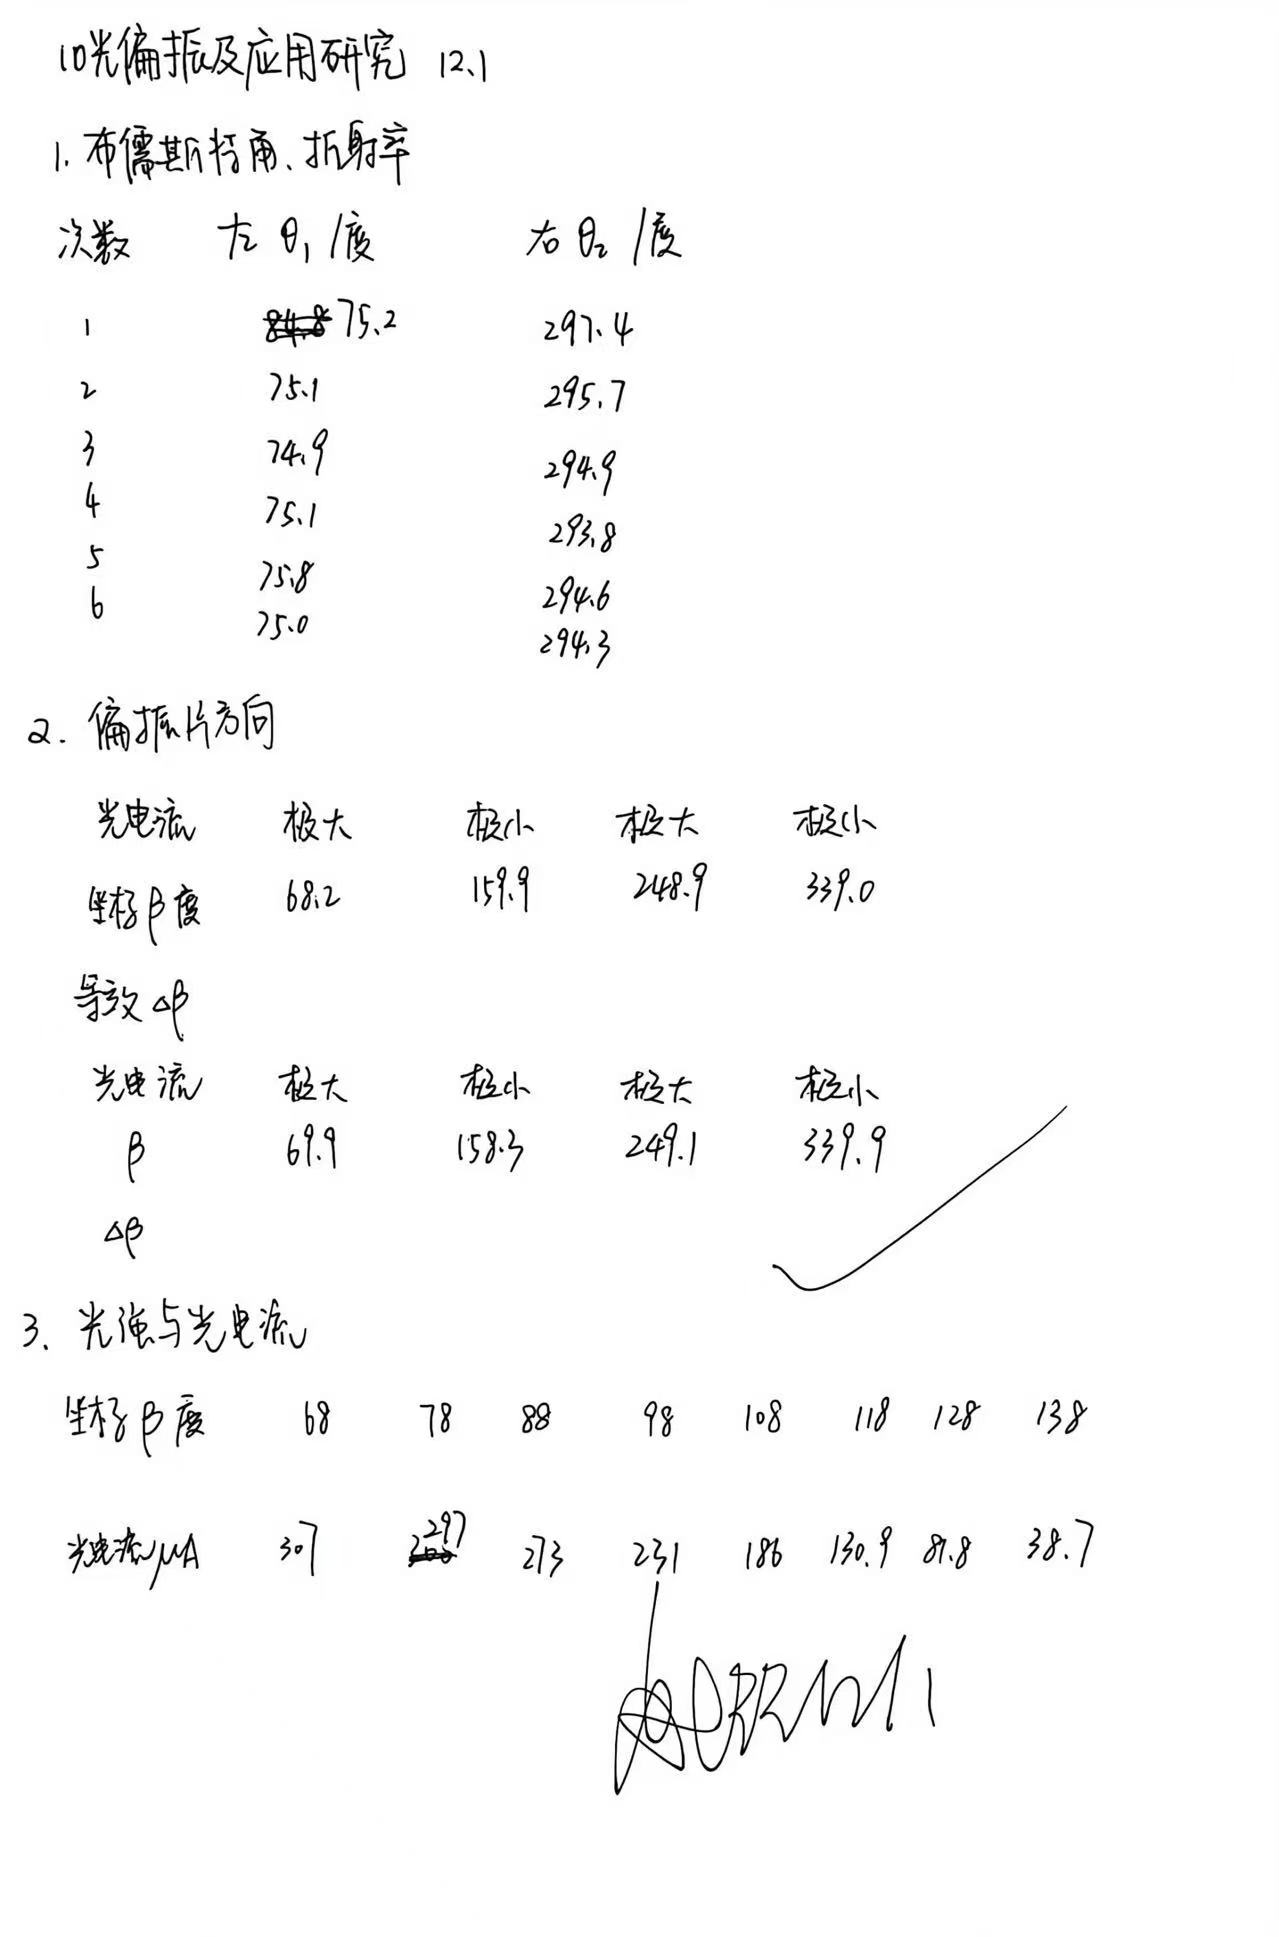
\includegraphics[width = 0.7\textwidth]{data.jpg}
\end{figure}

\FloatBarrier

\section{结果与分析（60分）}
\subsection{数据处理与结果（30分）}

\textbf{1.测量黑色平板的折射率}

将激光源调至最弱后，转动黑色平板，改变入射角，当探测器探测到的反射光的光电流极小时，记录转动臂的角坐标，
进行六次测量，每次包括左边和右边以消除转动臂刀口偏差：

\begin{table}[htbp!]
    \centering
\begin{tabular}{|l|l|l|}
    \hline
    测量次数 & 左侧角坐标 $\theta_1 /$ 度 & 右侧角坐标 $\theta_2 /$ 度 \\
    \hline
    1 & 75.2 & 297.4 \\
    \hline
    2 & 75.1 & 295.7 \\
    \hline
    3 & 74.9 & 294.9 \\
    \hline
    4 & 75.1 & 293.8 \\
    \hline
    5 & 75.8 & 294.6 \\
    \hline
    6 & 75.0 & 294.3 \\
    \hline
\end{tabular}
\end{table}

根据公式：
\[
\alpha = \frac{1}{4} |\theta_1 - \theta_2|
\]

计算黑色平板的布儒斯特角：
\begin{table}[htbp!]
    \centering
    \begin{tabular}{|l|l|l|l|l|l|l|}
        \hline
        $\alpha_1$ & $\alpha_2$ & $\alpha_3$ & $\alpha_4$ & $\alpha_5$ & $\alpha_6$ & $\bar{\alpha}$ \\
        \hline
        55.6 & 55.2 & 55.0 & 54.7 & 54.7 & 54.8 & 55.0 \\
        \hline
    \end{tabular}
\end{table}

因此有：
\[
\bar{n} = \tan{\bar{\alpha}} = 1.42
\]

计算折射率 $n$ 的不确定度，由于它与布儒斯特角 $\alpha$ 成非线性关系，
因此先计算布儒斯特角的不确定，包括多次测量导致的 $A$ 类不确定度：
\[
u_A(\alpha) = \sqrt{\frac{1}{N(N - 1)} \sum_{i=1}^N (\alpha_i - \bar{\alpha})^2} = 0.1348 ° , \quad N = 6
\]

以及仪器允差导致的 $B$ 类不确定度：
\[
u_B(\alpha) = \frac{\Delta \theta_仪}{\sqrt{3}} = 0.289 °
\]

黑色平板的布儒斯特角的总不确定度为：
\[
u(\alpha) = \sqrt{u_A^2(\alpha) + u_B^2(\alpha)} = 0.319 °
\]

根据折射率的不确定度传播公式，黑色平板的折射率的不确定度为：
\[
u(n) = (1 + n^2) \cdot u(\alpha) = 0.02
\]

最后黑色平板的折射率为：
\[
n = \bar{n} \pm u(n) = 1.42 \pm 0.02
\]

\textbf{2.标定偏振片的偏振化方向}

调整黑色平板的位置，使得激光以布儒斯特角入射，转动偏振片，记录透过光的光电流处于极值时偏振片指针的角坐标：

\begin{table}[htbp!]
    \centering
\begin{tabular}{|l|l|l|l|l|}
    \hline
    光电流 & 极大 & 极小 & 极大 & 极小 \\
    光电流极值处角坐标 $\beta /$ 度 & 68.2 & 159.9 & 248.9 & 339.0 \\
    偏振化方向与指针的等效夹角 $\Delta \beta /$ 度 & 68.2 & 69.9 & 68.9 & 69.0 \\
    \hline
    光电流 & 极大 & 极小 & 极大 & 极小 \\
    光电流极值处角坐标 $\beta /$ 度 & 69.9 & 158.3 & 249.1 & 339.9 \\
    偏振化方向与指针的等效夹角 $\Delta \beta /$ 度 & 69.9 & 68.3 & 69.1 & 69.9 \\
    \hline
\end{tabular}
\end{table}
\FloatBarrier

计算偏振化方向与指针的等效夹角的平均值：
\[
\bar{\Delta \beta} = 69.2 °
\]

这里的不确定度由 $A$ 类不确定度替代：
\[
u(\Delta \beta) = \sqrt{\frac{1}{N(N-1)} \sum_{i=1}^N (\Delta \beta_i - \bar{\Delta \beta})^2} = 0.3 ° , \quad N = 8
\]

因此偏振片的偏振化方向与偏振片指针的夹角为：
\[
\Delta \beta = (69.2 \pm 0.3)°
\]

\textbf{3.研究光电池的光电流与入射光强之间的关系}

从之前测量得到的偏振片的偏振化方向与指针的夹角附近开始旋转偏振片，等间隔记录光电流大小：

\begin{table}[htbp!]
    \centering
\begin{tabular}{|l|l|l|l|l|l|l|l|l|}
    \hline
    偏振片指针 $\beta /$ 度 & 68.0 & 78.0 & 88.0 & 98.0 & 108.0 & 118.0 & 128.0 & 138.0 \\
    \hline
    光电流 $i / \mu A$ & 307 & 297 & 273 & 231 & 186 & 130.9 & 81.8 & 38.7 \\
    \hline
    旋转角度 $\phi /$ 度 & -1.2 & 8.8 & 18.8 & 28.8 & 38.8 & 48.8 & 58.8 & 68.8 \\
    \hline
\end{tabular}
\end{table}

使用MATLAB作出光电流 $i$ 与 $\cos^2 \phi$ 的拟合曲线：
\begin{figure}[htbp!]
    \centering
    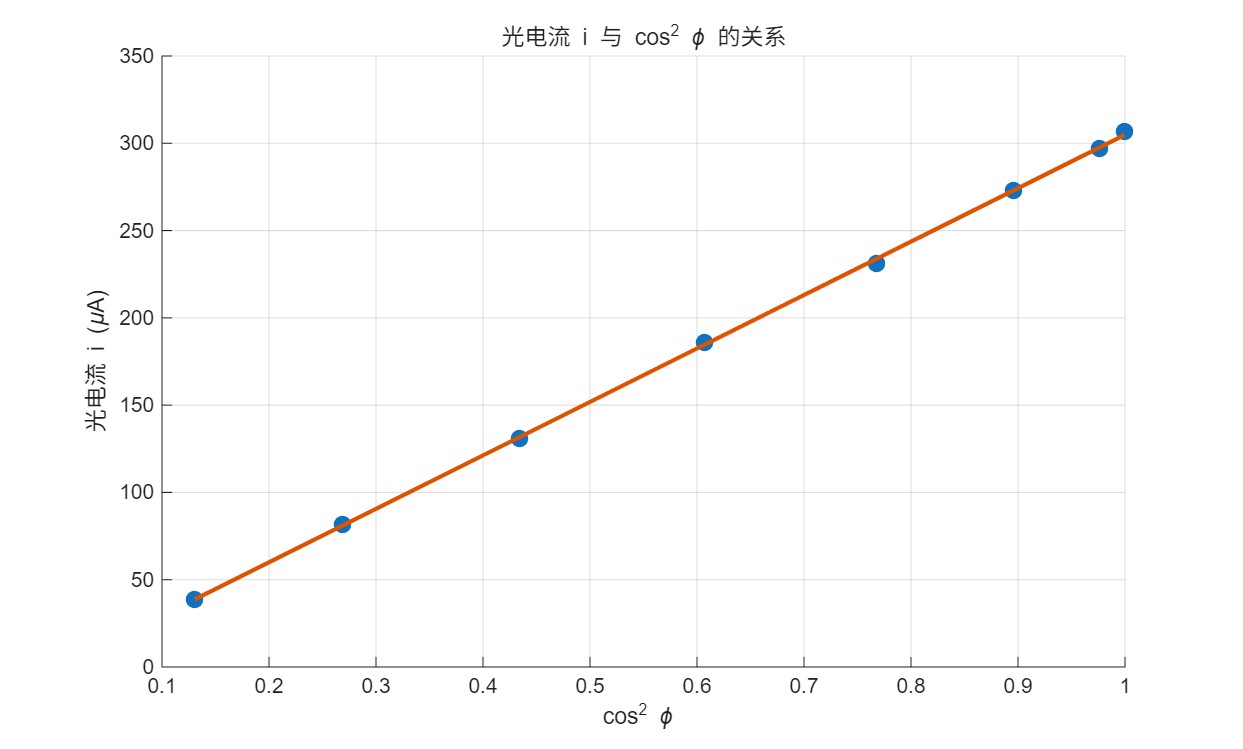
\includegraphics[width=0.7\textwidth]{q3_result.jpg}
\end{figure}

\FloatBarrier

从图中可以看出 $i$ 与 $\cos^2 \phi$ 基本呈线性关系，根据马吕斯定律可知入射光强 $I$ 正比于 $\cos^2 \phi$ ，
因此可知光电流 $i$ 与入射光强 $I$ 呈线性关系。


\subsection{误差分析（20分）}

在测量黑色平板的折射率和偏振片的偏振化方向时，$A$ 类不确定相对小，说明多次测量比较稳定；
在研究硅光电池的光电流和入射光强的关系时，两者基本满足线性关系，验证了光电流与入射光强的关系。

分析实验误差的主要来源：
\begin{enumerate}
    \item 测量激光入射角和偏振片方向的角度测量仪精度相对低，导致角度误差，并且由于非线性关系计算折射率时误差会放大；
    \item 万用表的光电流示数精度较低，无法完全准确判断极小值，增加了测量误差；
    \item 激光光源有波动，或者环境中的背景光干扰，导致光电流读数不稳定，角度极值的判断不完全准确。
\end{enumerate}

\subsection{实验探讨（10分）}

本实验探究了光的偏振特性及应用，并据此以激光为光源，借助光强探测器，测量了材料的布儒斯特角、折射率和偏振片的偏振化方向，
以及验证了马吕斯定律，说明了光电流与入射光强的线性关系。结果基本合理，误差较小。

\section{思考题（10分）}

\textbf{1. 请简述减小实验误差的方法。}

首先在实验前对仪器进行准直，确保光路尽量在同一水平高度，尽量打在黑色平板、偏振片及光强探测器中心；
其次就是在测量黑色平板的布儒斯特角时，测量转动臂在左右两侧的极小值并作差，消除转动臂刀口的偏差；
再次，对同一个量多次测量并取平均值，减小随机误差；
此外，尽量减小环境干扰，避免强背景光、减少振动、保持光学元件清洁等。


\textbf{2. 如何调节激光通过转台的中心转轴？}

首先调节激光器的高度和水平位置，使光束大致落在转台中心附近;接下来通过观察光斑落在转台附件的位置，微调激光器的左右以及前后位置，使光斑恰好落在黑色平板中心，并且反射光刚好能回到光源。
为验证光线是否真正通过转台中心转轴，可将转台旋转小角度，如果黑色平板上的光斑基本保持不移动或移动极小，则说明激光通过了中心轴；若光斑随旋转产生明显偏移，
则需继续微调激光器的水平位置与高度，重复上述步骤直至光斑在转台旋转过程中基本保持不变。

\textbf{3. 如何调节激光与转台转轴中心轴垂直？}

首先粗调激光器的高度，使激光大致入射黑色平板中心位置，若激光与转轴垂直，则反射光会沿原路径返回，若不垂直，则反射光会偏离原路径；
接下来通过微调激光器的水平朝向，使反射光尽可能返回光源方向，从而确保激光方向与镜面法线一致；然后将转台选择小角度，若激光与转轴垂直，
则反射光的位置应基本保持不变，若反射点移动明显，则说明激光仍未与转轴完全垂直，需要继续微调。

\begin{thebibliography}{9}
    \bibitem{ref1}
    赵航,郝彦军,朱俊,等. 光的偏振特性研究[J]. 实验科学与技术,2015(6):1-2. DOI:10.3969/j.issn.1672-4550.2015.06.001. 
    
    \bibitem{ref2}
    陈方平,祁铮. 布儒斯特角的测量方法[J]. 物理实验,2012,32(11):41-43. DOI:10.3969/j.issn.1005-4642.2012.11.010.    

\end{thebibliography}

\input{注意事项}
\end{document}
